\section{پردازش سیگنال و الگوریتم‌های استخراج نرخ ضربان قلب}
\label{sec:signal-processing-hr-estimation}

در این بخش، زنجیره‌ی پردازش سیگنال از نمونه‌برداری تا تخمین نرخ ضربان قلب (\lr{HR}) و استخراج ضرباهنگ قلب برای تحلیل \lr{HRV} شرح داده می‌شود. فرایند شامل مراحل زیر است:


\begin{figure}[ht]
    \centering
    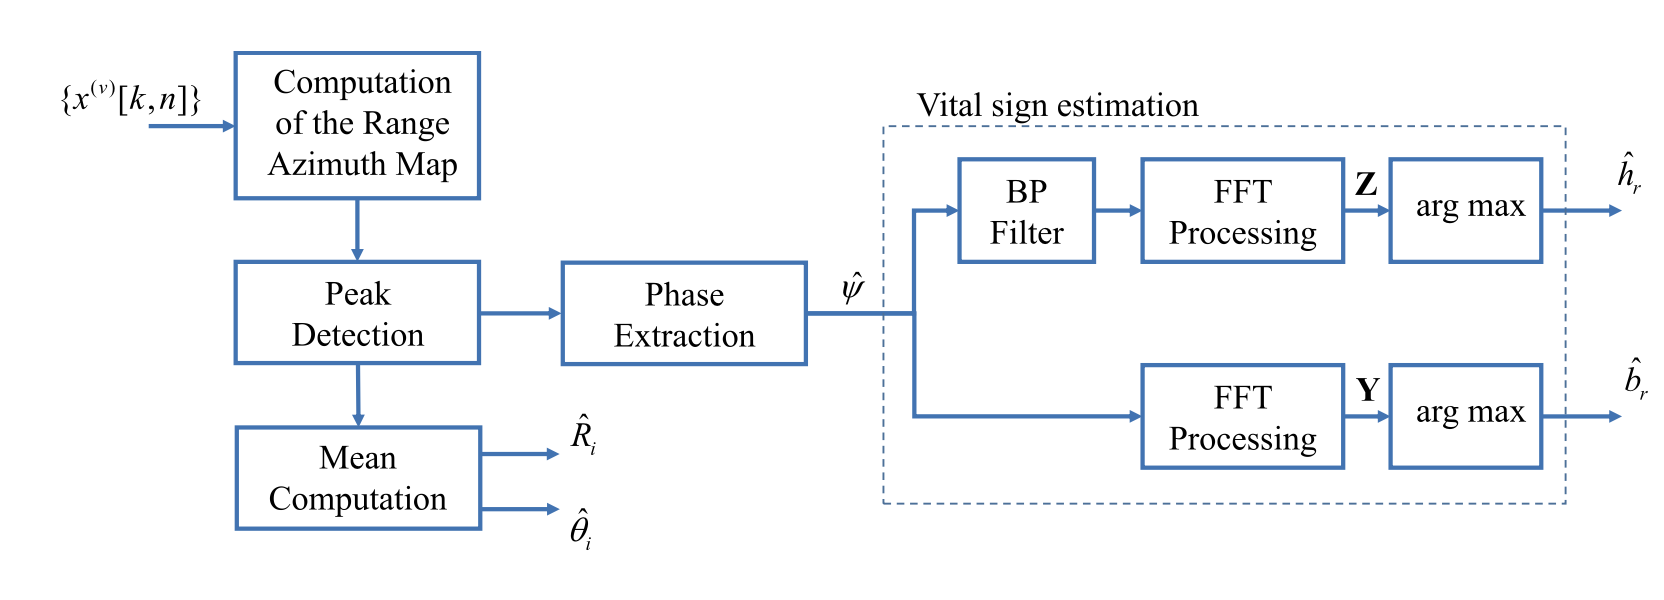
\includegraphics[width=0.7\linewidth]{Images/chapter3/3-3.png}
    \caption{
   نمایش پردازش سیگنال علائم حیاتی \lr{(HR و BR)} چندین نفر با استفاده از یک رادار \lr{MIMO} با موقعیت مکانی مشترک.
    \cite{paterniani2023radar}.}
    \label{fig:fmcw_vitals}
\end{figure}


\subsection{استخراج سیگنال میانی (\lr{Beat Signal}) و کالیبراسیون \lr{DC}}
\label{sec:beat-signal-dc-calibration}

پس از دریافت داده‌های \lr{IF} از مبدل آنالوگ‌به‌دیجیتال، یک \lr{FFT} مختصر (\lr{Slow-Time FFT}) روی هر چیپ انجام می‌شود تا فرکانس مناسب (\lr{bin}) مربوط به بازتاب از قفسه‌ی سینه انتخاب گردد. سپس سیگنال‌های \lr{I/Q} متناظر با آن \lr{bin} برای مراحل بعدی استخراج می‌شود.

از آنجا که خطاهای ساختاری ناشی از عدم تقارن \lr{I/Q} و \lr{DC Offset} می‌تواند موجب انحراف در فاز استخراجی شود، ابتدا با روش \lr{Least-Squares Circle Fitting} مؤلفه‌های \lr{DC} مجزای \lr{I} و \lr{Q} برآورد و حذف می‌شوند. با این کار، شکل موج فازِ استخراج‌شده به بازتاب واقعی سیگنال ضربان قلب نزدیک‌تر می‌گردد.


\subsection{استخراج فاز و آشفتگی‌زدایی (\lr{Phase Unwrapping})}
\label{sec:phase-unwrapping}

برای به‌دست آوردن فاز پیوسته‌ی حرکت قفسه‌ی سینه، از تابع آرکتانژانت دو متغیره استفاده می‌شود:

\begin{equation}
\phi[n] = \operatorname{atan2}(Q[n],\, I[n])
\label{eq:phase_extraction}
\end{equation}
\addequation{استخراج فاز از مؤلفه‌های \lr{I} و \lr{Q} با تابع آرکتانژانت دوارگشتی}

که خروجی در بازه $-\pi$ تا $\pi$ قرار دارد. سپس برای حذف جهش‌های ناخواسته بزرگ‌تر از $\pi$، الگوریتم \lr{Unwrapping} اجرا می‌شود. برای مواردی که جابجایی دیواره بیش از نیم طول موج باشد و \lr{Unwrapping} ساده خطا دهد، می‌توان از الگوریتم \lr{DACM (Differencing and Augmented Cross-Multiplication)} بهره برد.

\subsection{تقویت اجزاء ضربان قلب و حذف درفت فاز}
\label{sec:phase-detrend}

در سیگنال \lr{Unwrapped Phase}، مؤلفه‌های تنفسی با بازه‌ی فرکانسی بین 0.1 تا 0.5~\lr{Hz} معمولاً غالب‌تر از مؤلفه‌های ضربان قلب در بازه‌ی 0.8 تا 2.0~\lr{Hz} هستند. برای تقویت مؤلفه‌های ضربان، ابتدا تفاضل مرکزی فاز (بین نمونه‌های جلو و عقب) محاسبه می‌شود تا شیب‌های لحظه‌ای برجسته شوند:

\begin{equation}
\Delta \phi[n] = \phi[n+1] - \phi[n-1]
\label{eq:phase_diff}
\end{equation}
\addequation{محاسبه تفاضل مرکزی برای حذف روند و تقویت مولفه‌های پرنوسان مانند ضربان قلب}

در مواردی که مقدار تفاضل از آستانه‌ای بیش از حد بزرگ یا کوچک‌تر از منفی آستانه باشد، نمونه‌ها با درون‌یابی خطی اصلاح می‌شوند تا ناهمواری‌های ضربه‌ای (\lr{Impulse Noise}) برطرف گردد.

\subsection{فیلترینگ ناظر بر جداسازی بلوک‌های تنفس و ضربان}
\label{sec:bandpass-filtering}

پس از تفاضل فاز، دو فیلتر \lr{Bandpass IIR} مجزا اعمال می‌شود:

\begin{itemize}
  \item \lr{فیلتر دومرحله‌ای}: برای تفکیک مؤلفه‌های تنفسی در بازه‌ی فرکانسی \lr{0.1–0.5 Hz}
  \item \lr{فیلتر چهارمرحله‌ای}: برای جداسازی ضربان قلب در بازه‌ی \lr{0.8–2.0 Hz}
\end{itemize}

این ساختار به شکل بلادرنگ روی سیگنال اعمال و خروجی هر فیلتر برای مراحل بعدی نگهداری می‌شود.

\subsection{حذف اعوجاج ناشی از حرکت و کنترل بهره}
\label{sec:motion-artifacts}

برای مقابله با تداخل ناشی از حرکت‌های بزرگ بدن (\lr{Motion Corruption})، انرژی هر بخش یک‌ثانیه‌ای سیگنال ضربان قلب محاسبه می‌شود و با آستانه‌ای مقایسه می‌گردد:

\begin{equation}
E = \sum_{n=1}^{N} x^2[n]
\label{eq:energy}
\end{equation}
\addequation{محاسبه انرژی سیگنال در یک بازه زمانی به‌منظور شناسایی حرکت‌های ناخواسته}

در صورت عبور از آستانه، سیگنال مقیاس شده یا حذف می‌شود تا از ورود نویزهای حرکتی به تخمین جلوگیری گردد.

\subsection{ شناسایی پیک طیفی برای تخمین ضربان قلب}
\label{sec:peak-counting}

برای استخراج \lr{HR}، یک \lr{FFT} روی بخش‌های سالم خروجی فیلتر ضربان اجرا شده و قله‌ی طیفی متناظر با فرکانس قلب شناسایی می‌شود. تعداد پیک‌های متوالی در بازه‌ی زمانی مشخص، معادل نرخ ضربان قلب بر حسب \lr{bpm} است.

\subsection{تحلیل زمان فرکانس (\lr{STFT})}
\label{sec:stft}

به‌منظور ردیابی تغییرات لحظه‌ای ضربان و جداسازی بهتر هارمونیک‌های تنفس، از روش \lr{Short-Time Fourier Transform (STFT)} استفاده می‌شود. در هر پنجره‌ی زمانی، انرژی ترکیبی سیگنال به‌صورت زیر محاسبه می‌گردد:

\begin{equation}
E[n] = |x[n]|^2 + |y[n]|^2
\label{eq:stft_energy}
\end{equation}
\addequation{محاسبه انرژی در تحلیل \lr{STFT} برای تشخیص بازتاب‌های قوی از سطح بدن}

نقاط با بیشترین انرژی، بازتاب‌های ضربان قلب تلقی شده و تحلیل ادامه می‌یابد.

\subsection{الگوریتم \lr{Health-VMD} برای استخراج دقیق \lr{HRV}}
\label{sec:health-vmd}

برای تخمین \lr{HRV} نیاز به تشخیص دقیق هر ضربان (\lr{IBI}) است. در مقاله‌ی \lr{Health-Radar}، روش \lr{Variational Mode Decomposition (VMD)} با پارامترهای بهینه‌سازی‌شده توسط الگوریتم \lr{GOA (Grasshopper Optimization Algorithm)} پیشنهاد شده است. تابع هدف پیشنهادی:

\begin{equation}
\mathrm{PME} = \alpha \cdot H_{\mathrm{PE}} + \beta \cdot I_{\mathrm{MI}} + \gamma \cdot L_{\mathrm{Loss}}
\label{eq:pme_objective}
\end{equation}
\addequation{تابع هدف ترکیبی برای \lr{VMD} شامل آنتروپی جایگشتی، اطلاعات متقابل و نرخ اتلاف انرژی}


این روش تضمین می‌کند که هارمونیک‌های تنفس وارد مدهای ضربان نشوند. خروجی این الگوریتم، تخمین دقیق پارامترهایی نظیر \lr{SDNN} و \lr{RMSSD} است، با دقتی برابر:

\begin{equation}
\mathrm{RMSE} \approx 4.1\ \mathrm{ms}
\label{eq:rmse_sdnn}
\end{equation}
\addequation{خطای میانگین مربعی در تخمین \lr{SDNN} توسط الگوریتم \lr{Health-VMD}}

\subsection*{خلاصه‌ی نتایج}
\label{sec:summary}

با ترکیب مراحل فوق کالیبراسیون \lr{DC}، استخراج و \lr{Unwrapping} فاز، تفاضل و فیلترینگ \lr{IIR}، حذف آرتیفکت‌های حرکتی، \lr{STFT} و \lr{Health-VMD} دقت تخمین \lr{HR} به‌صورت زیر گزارش شده است:

\begin{equation}
\mathrm{MAE} < 2\ \mathrm{bpm},\quad \mathrm{RMSE_{HRV}} \approx 5\ \mathrm{ms}
\label{eq:hr_final_results}
\end{equation}
\addequation{دقت نهایی زنجیره‌ی پردازش در تخمین \lr{HR} و \lr{HRV} در شرایط بالینی}
